\subsection{Similar products}
Before we started exploring the options and benefits of development, we explored similar products for inspiration and in the hope of finding functionality possibilities that can easily be integrated in our product---functionalities nice to have but may not necessarily have been specified by a customer. Besides, the team thought exploring existing software solutions could help us learn something which is going to be new and some which were already tried. General opinions are that commercial-off-the-shelf software are thought to be straight forward, time and cost saving even thought it might bring its own version of problems\cite{similarproduct:introdn}. Having said that, we summarized the apps we tried and described some of them that were closer to the system we are trying to develop.
\paragraph{Project Noah - Networked Organisms and Habitats}

Project Noah is a mobile application that helps nature lovers discover local wildlife and aspiring citizen scientists contribute to current research  projects. Noah stands for networked organisms and habitats. It is a tool people can use to document and learn about their  natural surroundings and as a technology platform research groups can  use to harness the power of citizen scientists everywhere. And it documents species sighting with date, category, habitat, picture and comments\cite{similarproduct:noah}.

\begin{figure}[htb]
    \centering
    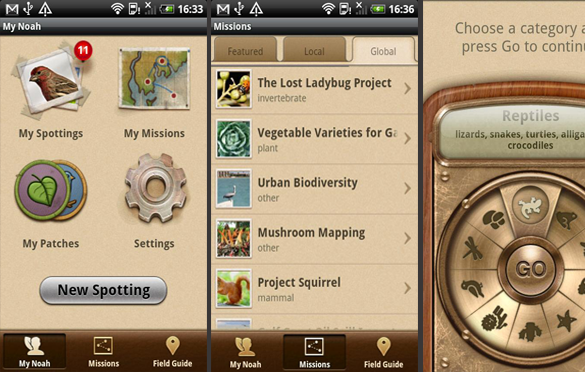
\includegraphics[width=0.8\textwidth]{introduction/project_description/noah.png}
    \caption{Projet Noah app}
    \label{fig:Noahapp}
\end{figure}

\paragraph{US Birding Checklist}
This is a bird watching tool set which records species sex, age location and pictures\cite{similarproduct:usbird}.

It uses an online database system called eBirds\cite{similarproduct:ebird}, which is launched and run by Cornell Lab of Ornithology and National Audubon Society. It also show the distribution of birds on a map.

\begin{figure}[htb]
    \centering
    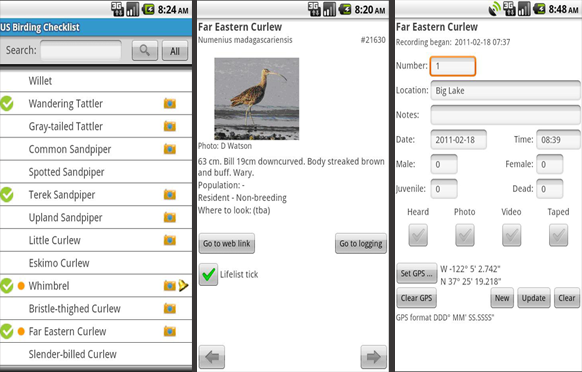
\includegraphics[width=0.8\textwidth]{introduction/project_description/usbirdingchecklist.png}
    \caption{US Bird Checklist app}
    \label{fig:usbirdapp}
\end{figure}

\paragraph{Audubon Guide}
Audubon is a portable dictionary like content provision on mobile phones. It downloads a wealth of information about mammals, birds, butterflies and more on the mobile phone and its focus is for viewing and providing information about species\cite{similarproduct:audubon}. Audubon has a variety of version such as Audubon Wildflowers, Audubon Butterflies, Audubon Mammals.

\begin{figure}[htb]
    \centering
    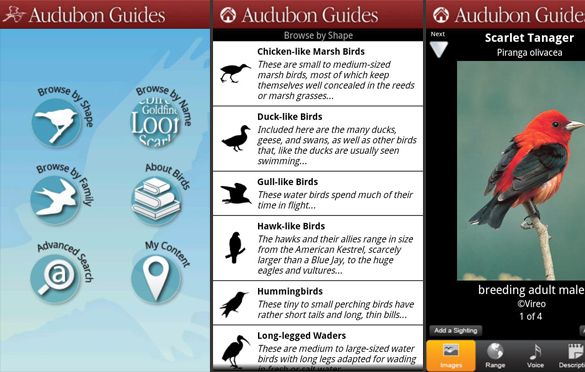
\includegraphics[width=0.8\textwidth]{introduction/project_description/audubonguide.png}
    \caption{Audubon species guide app}
    \label{fig:audubonapp}
\end{figure}

But we found none of the application fit for the requirements from Artsdatabanken. Artsdatabanken runs its own data source and whatever COTS the team considers should enable Artsdatabaken to access its data source. Artsdatabanken requirements recommend a strict inclusion of requirements such as inclusion of location, pictures, number of species, activity which are handled in a different ways in the applications described above. The applications are also not free and  cannot be customized to our customer's needs, a lot more reason to resort to development. It is at point that we decided that development is the only option to fulfill our customers's requirements.

